\documentclass[aspectratio=169,10pt]{beamer}
\usetheme{Madrid}
\usecolortheme{seahorse}
\usefonttheme{professionalfonts}

\setbeamertemplate{footline}[frame number]
\setbeamertemplate{navigation symbols}{}

\usepackage{graphicx}
\graphicspath{{figures/}}
\usepackage{amsmath,amssymb,mathtools}
\usepackage{booktabs}
\usepackage{listings}
\usepackage{xcolor}
\usepackage{tikz}

\lstset{
  basicstyle=\ttfamily\scriptsize,
  numbers=left,
  numberstyle=\tiny,
  frame=single,
  backgroundcolor=\color{gray!7},
  commentstyle=\color{green!50!black}\itshape,
  keywordstyle=\color{blue}\bfseries,
  stringstyle=\color{orange},
  breaklines=true,
  showstringspaces=false,
  language=Python
}

\newcommand{\Rmb}{\mathbb{R}}
\newcommand{\Pmb}{\mathbb{P}}
\newcommand{\Emb}{\mathbb{E}}
\newcommand{\Qmb}{\mathbb{Q}}
\newcommand{\Nmb}{\mathbb{N}}

\title[E-Values -- Ch.7]{Hypothesis Testing with E-Values}
\subtitle{Chapter 7: Sequential Anytime-Valid Inference using E-Processes}
\author{Based on Ramdas \& Wang}
\date{}

\begin{document}

\begin{frame}
\titlepage
\end{frame}

\begin{frame}{Outline}
\tableofcontents
\end{frame}

% ==========================================================================
\section{Background you need}
% ==========================================================================

\begin{frame}[allowframebreaks]{Notation and background you need}

This chapter is entirely about \emph{sequential} data: $X_1, X_2, X_3, \dots$ arriving one at a time.
Everything hinges on four ideas that are new if you have only seen fixed-sample-size statistics.
We build each one from scratch with a plain-English analogy first, then the formal definition.

\vspace{0.3cm}
\textbf{(a) Filtration --- your growing folder of evidence.}

\emph{Intuition:} Imagine a folder that only ever gains pages. Page $t$ contains everything you knew right after
seeing the $t$-th data point. You can look back at old pages any time, but you can never un-see what is already
inside, and you cannot peek at future pages. A \emph{filtration} $(\mathcal{F}_t)_{t \in \mathbb{T}}$ is the mathematical
version of this folder: a nested, non-decreasing sequence of $\sigma$-algebras,
$$\mathcal{F}_0 \subseteq \mathcal{F}_1 \subseteq \mathcal{F}_2 \subseteq \cdots,$$
where $\mathcal{F}_t$ represents ``all events you can decide are true or false using only data up to time $t$.''
Usually $\mathcal{F}_t = \sigma(X_1,\dots,X_t)$, the \emph{natural filtration} generated by the data itself,
with $\mathcal{F}_0 = \{\varnothing,\Omega\}$ (trivial --- you know nothing yet). A process $Y = (Y_t)$ is
\emph{adapted} to $\mathcal F$ if $Y_t$ is measurable w.r.t.\ $\mathcal{F}_t$ for every $t$ --- informally, $Y_t$ is
computable from data available by time $t$, no peeking ahead allowed. A process is \emph{predictable} if $Y_t$ is
measurable w.r.t.\ $\mathcal{F}_{t-1}$ --- it must be decided \emph{before} seeing $X_t$.

\framebreak

\textbf{(b) Stopping time --- a rule for when to stop looking.}

\emph{Intuition:} You are flipping a coin and you decide: ``I'll stop the very first time I see 3 heads in a row.''
This is a legitimate rule because, at every moment, you can tell (using only what you've seen so far) whether to
stop right now. Contrast this with an illegitimate rule like ``I'll stop one flip before the 10th head'' --
you cannot know in advance which flip that is without seeing the future.

A \emph{stopping time} $\tau$ is a random variable taking values in $\{0,1,2,\dots\} \cup \{\infty\}$ such that
$$\{\tau \le t\} \in \mathcal{F}_t \quad \text{for every } t.$$
In words: at every time $t$, you can decide (using only $\mathcal{F}_t$, i.e., data so far) whether the rule has
told you to stop by now. Stopping times formalize ``peeking at the data and deciding to stop'' --- as long as the
decision to stop at time $t$ only uses information available at time $t$.

\framebreak

\textbf{(c) Supermartingale --- wealth in a game rigged against you (or fair, at best).}

\emph{Intuition:} Think of $M_t$ as your wealth after $t$ rounds of a betting game. A \emph{supermartingale} means:
given everything you know so far, your expected wealth tomorrow is at most your wealth today. The game may be
unfavorable or exactly fair, but never favorable, on average, one step ahead.

Formally, $M = (M_t)$ is a supermartingale for $\mathbb{P}$ if it is adapted, integrable, and
\begin{block}{Supermartingale}
$$\mathbb{E}^{\mathbb{P}}[M_t \mid \mathcal{F}_{t-1}] \le M_{t-1} \quad \text{for all } t \ge 1.$$
\end{block}
If ``$\le$'' is replaced by ``$=$'', $M$ is a \emph{martingale} (a perfectly fair game). A \emph{test
(super)martingale} for a set of nulls $\mathcal{P}$ additionally requires: $M_t \ge 0$ a.s.\ for every
$\mathbb{P} \in \mathcal{P}$, and $\mathbb{E}^{\mathbb{P}}[M_0] \le 1$.

\framebreak

\textbf{(d) E-process --- your wealth betting against the null.}

\emph{Intuition:} Start with \$1. At every step you place a bet against the null hypothesis being true. If the null
is true, your bet is designed so you cannot expect to profit (on average, wealth does not grow); if the null is
false, a good strategy lets your wealth grow, potentially to enormous multiples of your starting \$1. The path of
your wealth over time is the \emph{e-process}. Large wealth at any point you choose to stop and look is evidence
against the null.

\begin{block}{E-process (Definition 7.3)}
A sequence $E = (E_t)_{t\in\mathbb T}$ adapted to $\mathcal F$ is an e-process for $\mathcal P$ if either
(equivalent) condition holds:
\begin{itemize}
\item[(a)] $\mathbb{E}^{\mathbb{P}}[E_\tau] \le 1$ for every stopping time $\tau$ and every $\mathbb{P}\in\mathcal P$;
\item[(b)] there is a test martingale family $(M^{\mathbb P})_{\mathbb P \in \mathcal P}$ with $E \le M^{\mathbb P}$
a.s., for each $\mathbb P \in \mathcal P$.
\end{itemize}
\end{block}
Every test (super)martingale is an e-process, but not every e-process is a (super)martingale --- e-processes form
a strictly larger, more flexible class. This chapter's entire agenda is: build such wealth processes, and show they
give valid sequential tests \emph{no matter when or why you decide to stop}.

\framebreak

\textbf{Why this matters, in one sentence.} A fixed-sample-size test (e.g., a classical $p$-value at a
pre-announced $n$) is only guaranteed valid if you look at the data exactly once, at the $n$ you fixed in advance.
An e-process is a wealth process that stays a valid measure of evidence \emph{no matter which (random,
data-dependent) time $\tau$ you choose to stop and look} --- this is what ``anytime-valid'' means, and it is the
whole point of sequential anytime-valid inference (SAVI).

\end{frame}

% ==========================================================================
\section{7.1 The problematic practice of peeking at p-values}
% ==========================================================================

\begin{frame}[allowframebreaks]{7.1 Peeking at p-values: the problem}

\textbf{Intuition.} A scientist collects data one subject at a time and, being impatient (or economical), checks
the $p$-value after every few subjects. If it ever dips below $0.05$, she stops and declares victory. This feels
harmless --- after all, each individual $p$-value is a legitimate 5\%-level test. But looking at \emph{many} of them
and stopping at the first lucky dip is a completely different, and much riskier, procedure.

\vspace{0.2cm}
\textbf{Setup.} Suppose $P_1, P_2, \dots$ is a sequence of $p$-values computed after $1, 2, 3, \dots$ subjects
(assume for now each $P_n$ is exactly $\text{Uniform}(0,1)$ under the null, as classical theory promises). Define
the stopping time
$$\tau := \inf\{n \ge 1 : P_n \le \alpha\}.$$

\begin{block}{The heart of the issue}
Even though, for every \emph{fixed} $n$,
$$\mathbb{P}(P_n \le \alpha) \le \alpha,$$
it is typically the case (e.g., for a $t$-test $p$-value) that $\tau < \infty$ almost surely under the null, and
$$\mathbb{P}(P_\tau \le \alpha) = 1.$$
\end{block}

That is: if you are willing to wait long enough, you are \emph{guaranteed} to see a ``significant'' result, even
when the null is exactly true! This is called \textbf{sampling to a foregone conclusion}.

\framebreak

\textbf{Why does this happen?} A valid $p$-value guarantee, $\mathbb{P}(P_n \le \alpha) \le \alpha$, is a statement
about one fixed, pre-chosen $n$. It says nothing about the probability that \emph{some} $P_n$ along the way dips
below $\alpha$. Under the null, $P_n$ fluctuates forever (it does not converge to anything sensible), and a
fluctuating sequence started arbitrarily many times will eventually hit any fixed threshold with probability 1
(much like a symmetric random walk eventually crosses any level).

\textbf{Consequences.}
\begin{itemize}
\item This is believed to be a real contributor to the ``reproducibility crisis'' in psychology, biomedicine, and
social science: researchers who informally check their data as it accumulates (even with good intentions) can
inflate the true type-I error far above the nominal $\alpha$.
\item The problem cannot be diagnosed from the data alone --- you would need to know the exact protocol
(did they peek? how often?) to correct for it, and this information is rarely reported.
\item Rather than trying to \emph{ban} peeking (unenforceable), this chapter's approach is to design procedures
that remain valid \emph{no matter how or when} you peek. That is exactly what e-processes deliver.
\end{itemize}

\end{frame}

% ==========================================================================
\section{7.2 Wald's sequential probability ratio test}
% ==========================================================================

\begin{frame}[allowframebreaks]{7.2 Wald's SPRT: a motivating numerical example}

\textbf{Setup.} Data $X_1, X_2, \dots$ are iid $\text{Bernoulli}(p)$. Null: $p = 1/2$. Alternative: $p = 0.6$. Let
$f_0, f_1$ be the null/alternative densities. The likelihood ratio process is
\begin{block}{Likelihood ratio}
$$L_n = \prod_{i=1}^n \frac{f_1(X_i)}{f_0(X_i)}.$$
$L_n$ is an e-variable at each fixed $n$; the sequence $(L_t)_{t\in\Nmb}$ is in fact an e-process.
\end{block}

\textbf{Fixed-sample Neyman--Pearson LRT.} For target type-I error $\alpha=0.05$ and type-II error $\beta=0.05$, a
calculation shows $n=280$ and the optimal rule rejects when $L_{280} \ge \gamma = 0.962$ (equivalently, at least
154 heads out of 280). Curiously, $\gamma < 1$: we reject even though the alternative's likelihood is only
marginally larger than the null's.

\textbf{Wald's SPRT.} Instead of waiting for a fixed $n$, update $L_t$ after every observation:
\begin{itemize}
\item if $L_t \ge \gamma_1 = 1/\alpha$: reject the null and stop;
\item if $L_t \le \gamma_0 = \beta$: accept (fail to reject) and stop;
\item otherwise: keep sampling.
\end{itemize}
These conservative thresholds $\gamma_0=\beta,\ \gamma_1=1/\alpha$ keep type-I and type-II errors below $\alpha,\beta$
respectively, as a consequence of Ville's inequality (Section 7.4). For our numbers: reject if $L_t \ge 20$, accept
if $L_t \le 0.05$.

\framebreak

\begin{table}
\centering
\scriptsize
\begin{tabular}{lcccc}
\toprule
Data-generating dist. & $p=0.5$ & $p=0.55$ & $p=0.6$ & $p=0.65$ \\
Setting & null & misspecified & alternative & misspecified \\
\midrule
SPRT expected sample size & 137.7 & 234.5 & 139.3 & 76.1 \\
LRT pre-specified sample size & 280 & 280 & 280 & 280 \\
Power of SPRT & 0.04 & 0.52 & 0.96 & 1.00 \\
Power of LRT & 0.05 & 0.48 & 0.95 & 1.00 \\
\bottomrule
\end{tabular}
\caption{\scriptsize Comparison of SPRT vs.\ fixed-sample LRT (10,000 Monte Carlo repetitions). Table 7.1 of the text.}
\end{table}

\textbf{Punchline.} Under both the null and the alternative, the SPRT stops, on average, using roughly \emph{half}
the samples of the fixed-design LRT ($137.7$ or $139.3$ vs.\ $280$), while achieving comparable power. Sequential
testing is not just ``the same test done incrementally'' --- it can be dramatically more efficient.

\begin{block}{Theorem 7.2: Wald's SPRT optimality (informal)}
Let $\alpha,\beta$ be LRT errors with $n$ samples; let $\alpha',\beta'$ be SPRT errors with stopping time $\tau$.
If $\alpha \le \alpha'$ and $\beta \le \beta'$, then $\max(\mathbb{E}^{\mathbb P}[\tau], \mathbb{E}^{\mathbb Q}[\tau]) \le n$:
no other rule with equal or better error control needs a smaller expected sample size than the SPRT.
\end{block}

\framebreak

\textbf{How SAVI differs from Wald's classical paradigm (four points):}
\begin{enumerate}
\item \textbf{Decisions vs.\ evidence:} Wald wants a binary accept/reject decision with pre-set errors; SAVI wants
a continuously-updatable \emph{measure of evidence} (the e-process) --- decisions are a secondary, optional use.
\item \textbf{One stopping rule vs.\ all stopping rules:} Wald designs one specific stopping rule in advance; an
e-process is valid \emph{simultaneously at every possible stopping time}, planned or not.
\item \textbf{Optimality criteria differ:} Wald optimizes the error-vs.-sample-size tradeoff; SAVI's ``log-optimality''
(introduced below) optimizes the growth rate of evidence. For simple null/alternative these happen to coincide, but
not in general.
\item \textbf{Beyond likelihood ratios:} Wald's classical theory needs likelihood ratios to exist (parametric,
common reference measure). E-processes give a universal language that works for arbitrary composite, even
nonparametric, nulls.
\end{enumerate}

\end{frame}

\begin{frame}{Visualizing anytime-valid sequential testing under the alternative}

\textbf{Setup.} Bet on iid Bernoulli data using the likelihood-ratio strategy towards $q=0.6$ (factor $1.2$ on
heads, $0.8$ on tails), but now the \emph{true} bias is $p=0.6$ (the alternative is correct). The e-process should
grow exponentially on average, and we may stop and reject as soon as it crosses the rejection threshold
$1/\alpha$ --- we do not need to wait for a pre-specified sample size.

\begin{figure}
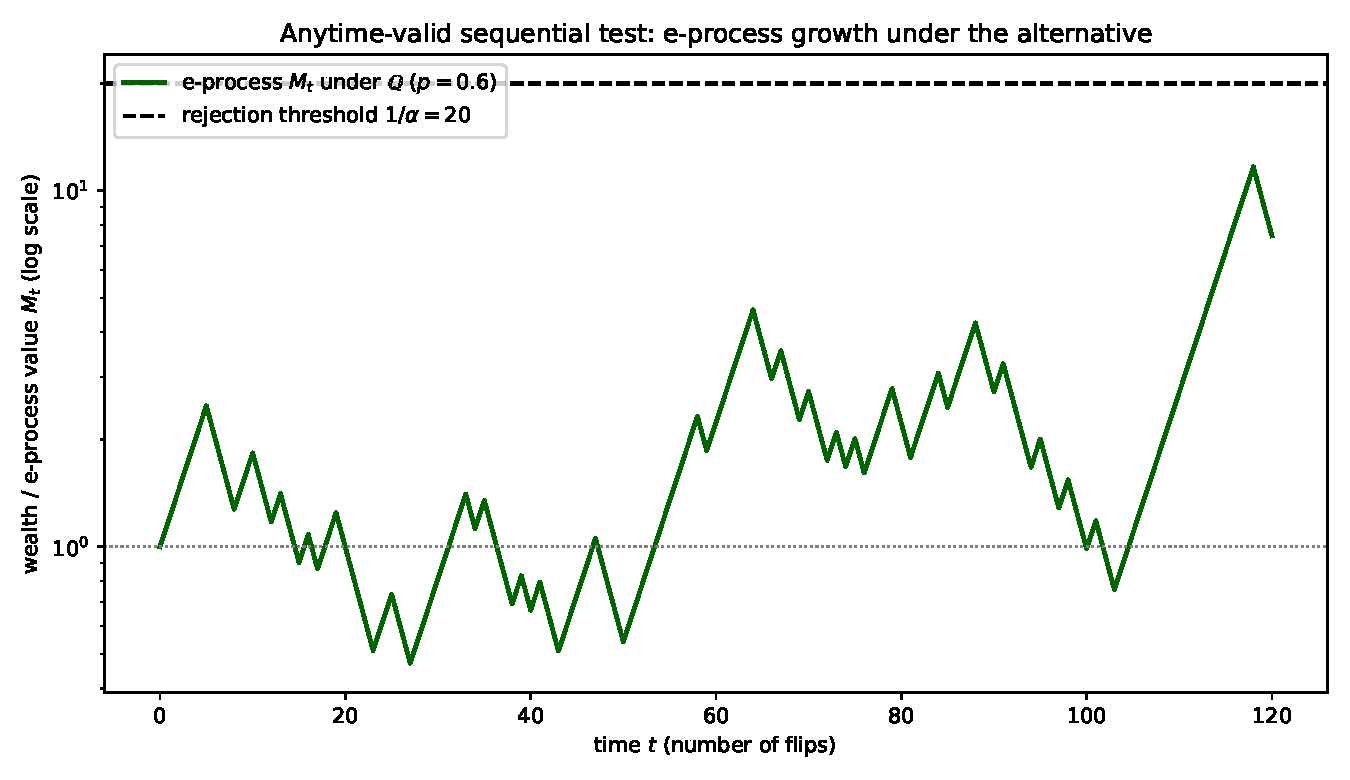
\includegraphics[width=0.52\textwidth]{eprocess_alt.pdf}
\end{figure}

The path fluctuates (bets can lose in the short run) but trends upward; here it first crosses the threshold
$1/\alpha = 20$ at $t=70$, at which point we may stop and reject $H_0$ --- exactly the anytime-valid analogue of
Wald's SPRT rejection rule from Section 7.2, but now understood as a special case of thresholding a general
e-process (Proposition 7.8).

\end{frame}

% ==========================================================================
\section{7.3 Test supermartingales, sequential tests, and e-processes}
% ==========================================================================

\begin{frame}{7.3 Four SAVI tools}

\textbf{Intuition.} There are four closely related objects for sequential inference; two are tied to a fixed
significance level $\alpha$ and two are not.

\begin{itemize}
\item \textbf{e-processes} (no fixed $\alpha$) --- our main object: sequential analog of e-variables.
\item \textbf{p-processes} (no fixed $\alpha$) --- sequential analog of p-variables.
\item \textbf{level-$\alpha$ sequential tests} --- sequential analog of level-$\alpha$ tests.
\item \textbf{$(1-\alpha)$-confidence sequences} --- sequential analog of confidence intervals.
\end{itemize}

We focus on e-processes: the others follow from Ville's inequality (next section) applied to one or more
e-processes.

\end{frame}

\begin{frame}{7.3 Level-$\alpha$ sequential tests}

\textbf{Intuition.} A sequential test is a rule that, at each time $t$, outputs a binary ``reject / don't reject''
decision $\phi_t \in \{0,1\}$ using only data so far, and once it rejects, it stays rejected. Validity means: the
chance you \emph{ever} falsely reject (across all of time) is at most $\alpha$.

\begin{block}{Level-$\alpha$ sequential test}
A binary adapted process $\phi = (\phi_t)$ is a level-$\alpha$ sequential test for $\mathcal P$ if
\begin{equation}
\sup_{\mathbb{P}\in\mathcal P} \mathbb{P}(\exists t \ge 1 : \phi_t = 1) \le \alpha.
\tag{7.1}
\end{equation}
\end{block}

Equivalently, letting $\tau := \inf\{t\ge 1 : \phi_t = 1\}$ (a stopping time; $\inf \varnothing = \infty$), the
condition becomes
\begin{equation}
\mathbb{E}^{\mathbb{P}}[\phi_\tau] \le \alpha \quad \text{for all } \mathbb{P}\in\mathcal P,\ \tau\in\mathcal T.
\tag{7.2}
\end{equation}
Here $\phi_t$: reject-or-not indicator at time $t$; $\mathcal T$: set of all $\mathcal F$-stopping times.

\end{frame}

\begin{frame}{7.3 Test (super)martingales and e-processes: formal definitions}

\begin{block}{Definition 7.3}
\textbf{(i)} $M=(M_t)_{t\in\mathbb T}$ is a \emph{test (super)martingale} for $\mathcal P$ if for every
$\mathbb P \in \mathcal P$: (a) $M \ge 0$ a.s.; (b) $M$ is a (super)martingale under $\mathbb P$; (c)
$\mathbb E^{\mathbb P}[M_0] \le 1$.

\textbf{(ii)} An e-process $E=(E_t)$ adapted to $\mathcal F$ satisfies either (equivalent):
\begin{itemize}
\item[(a)] $\mathbb E^{\mathbb P}[E_\tau] \le 1$ for any stopping time $\tau \in \mathcal T$, any $\mathbb P \in \mathcal P$;
\item[(b)] $\exists$ a test martingale family $(M^{\mathbb P})_{\mathbb P\in\mathcal P}$ with $E \le M^{\mathbb P}$
a.s., for each $\mathbb P$.
\end{itemize}
\end{block}

The equivalence of (a) and (b) is nontrivial (uses Doob's decomposition); we take it as given. Every test
(super)martingale is trivially an e-process (take $M^{\mathbb P}=M$), but the converse fails: e-processes are a
strictly larger, more flexible class.

\begin{block}{Definition 7.4: asymptotic growth rate}
An e-process $M$ is \emph{consistent} against $\mathbb Q$ if $M_t \to \infty$, $\mathbb Q$-a.s. The (typically
$\mathbb Q$-a.s.\ constant) quantity $\liminf_{t\to\infty} \frac{\log M_t}{t}$ is the \emph{asymptotic growth rate}
of $M$ against $\mathbb Q$. It is always $\le 0$ against $\mathbb{P} \in \mathcal P$.
\end{block}

\end{frame}

\begin{frame}[fragile]{Python: simulating a supermartingale}

We simulate a simple test martingale directly from Definition 7.3: bet on iid fair coin flips ($X_i \in \{0,1\}$)
using the likelihood-ratio bet towards $q=0.6$, i.e., multiply wealth by $1.2$ on heads and $0.8$ on tails.
Under the true null ($p=0.5$), this wealth process is a genuine \emph{martingale} (hence a supermartingale):
$\mathbb{E}[\text{next factor}] = 0.5(1.2) + 0.5(0.8) = 1$.

\begin{lstlisting}
import numpy as np

def simulate_wealth(n_steps, p_true, q=0.6, seed=0):
    rng = np.random.default_rng(seed)
    heads = rng.random(n_steps) < p_true
    factor = np.where(heads, 2*q, 2*(1-q))   # 1.2 if heads, 0.8 if tails
    wealth = np.concatenate(([1.0], np.cumprod(factor)))
    return wealth

# Under H0 (p=0.5): E[factor] = 0.5*1.2 + 0.5*0.8 = 1.0  -> martingale
w_null = simulate_wealth(400, p_true=0.5, seed=1)
print("wealth at t=400 under H0:", round(w_null[-1], 4))

# Check the martingale property empirically: average factor over many paths
factors = []
for s in range(20000):
    heads = np.random.default_rng(s).random(1) < 0.5
    factors.append(1.2 if heads[0] else 0.8)
print("empirical E[factor | H0] =", round(np.mean(factors), 4), " (theory: 1.0)")
\end{lstlisting}

\end{frame}

% ==========================================================================
\section{7.4 Optional stopping and Ville's inequality}
% ==========================================================================

\begin{frame}[allowframebreaks]{7.4 The optional stopping theorem}

\textbf{Intuition.} If wealth $M$ never grows in expectation one step ahead (a supermartingale), then no matter
which stopping time $\tau$ you pick to cash out --- even a rule that peeks at the whole history and cleverly
decides when to stop --- your expected wealth at that random time is still at most where you started. You cannot
out-smart a fair (or unfavorable) game by choosing \emph{when} to stop.

\textbf{Supermartingale convergence.} Any test supermartingale $M$ for $\mathbb{P}$ has a well-defined
(finite) $\mathbb{P}$-almost sure limit $M_\infty := \lim_n M_n$.

\begin{block}{Fact 7.5: Optional stopping theorem}
If $M$ is a test (super)martingale for $\mathbb P$, then for any stopping times $\sigma \le \tau$,
$$\mathbb{E}^{\mathbb{P}}[M_\tau \mid \mathcal F_\sigma] \le M_\sigma.$$
Taking $\sigma = 0$: $\mathbb{E}^{\mathbb P}[M_\tau] \le 1$. Consequently, if $M$ is an e-process for $\mathcal P$,
then $\mathbb E^{\mathbb P}[M_\tau] \le 1$ for all $\mathbb P \in \mathcal P$.
\end{block}

Notably, this version holds for \emph{any} stopping time $\tau$, with no boundedness restriction --- a consequence
of the nonnegativity of $M$.

\framebreak

\textbf{Intuition for Ville's inequality.} Combine optional stopping with Markov's inequality: since
$\mathbb E^{\mathbb P}[M_\tau] \le 1$ for \emph{every} stopping time $\tau$ (not just fixed times), we can bound the
probability that the wealth process \emph{ever} gets as large as $1/\alpha$ --- not just at one time, but over its
entire trajectory.

\begin{block}{Fact 7.6: Ville's inequality}
If $M$ is an e-process for $\mathcal P$, the following equivalent statements hold for every $\alpha \in [0,1]$:
\begin{equation}
\mathbb{P}\Big(\exists t \in \mathbb N : M_t \ge \tfrac{1}{\alpha}\Big) \le \alpha \quad \text{for every } \mathbb P \in \mathcal P;
\tag{Ville}
\end{equation}
\begin{equation}
\iff \sup_{\mathbb P\in\mathcal P}\mathbb{P}\Big(\sup_{t\in\Nmb} M_t \ge \tfrac1\alpha\Big) \le \alpha;
\tag{7.4a}
\end{equation}
\begin{equation}
\iff \sup_{\mathbb P\in\mathcal P,\,\tau\ge0}\mathbb{P}\Big(M_\tau \ge \tfrac1\alpha\Big)\le\alpha,\ \ \tau \text{ any stopping time}.
\tag{7.4b}
\end{equation}
\end{block}

\framebreak

\textbf{Step-by-step proof idea of Ville's inequality.}

\textbf{Step 1 (define the crossing time).} Fix $\alpha \in (0,1]$ and let
$$\tau^* := \inf\{t \ge 0 : M_t \ge 1/\alpha\}$$
(with $\inf \varnothing = \infty$). This is a valid stopping time: whether $\tau^* \le t$ depends only on
$M_0,\dots,M_t$, all $\mathcal F_t$-measurable.

\textbf{Step 2 (apply optional stopping at $\tau^*$).} By Fact 7.5 (optional stopping), for every finite $n$,
$$\mathbb E^{\mathbb P}[M_{\tau^* \wedge n}] \le \mathbb{E}^{\mathbb P}[M_0] \le 1,$$
since $M_{\tau^*\wedge n}$ is the wealth process stopped at the (finite, bounded) time $\tau^* \wedge n$, and stopped
supermartingales are still supermartingales.

\textbf{Step 3 (Markov's inequality on the event of crossing).} On the event $\{\tau^* \le n\}$, we have
$M_{\tau^*\wedge n} = M_{\tau^*} \ge 1/\alpha$ by definition of $\tau^*$ (assuming no ``jump over'' the threshold,
which holds since we check every integer time). Hence
$$\mathbb{P}(\tau^* \le n) \le \alpha\, \mathbb E^{\mathbb P}[M_{\tau^*\wedge n}] \le \alpha.$$

\textbf{Step 4 (let $n \to \infty$).} $\{\tau^* \le n\} \uparrow \{\tau^* < \infty\} = \{\exists t: M_t \ge 1/\alpha\}$,
so by continuity of probability,
$$\mathbb P(\exists t : M_t \ge 1/\alpha) = \lim_{n\to\infty}\mathbb P(\tau^*\le n) \le \alpha. \qquad \blacksquare$$

\framebreak

\textbf{Reading the inequality.} For any \emph{fixed} $t$, $M_t$ is itself an e-variable, so
$\mathbb P(M_t \ge 1/\alpha) \le \alpha$ is just ordinary Markov's inequality. Ville's inequality is the
\emph{time-uniform} generalization: the bound holds simultaneously across the entire (possibly infinite) trajectory,
not just at one time slice. This is exactly what makes stopping at a data-dependent time safe.

\textbf{Practical meaning.} Defining $\phi_t := \mathbb 1\{M_t \ge 1/\alpha\}$ turns $M$ into a level-$\alpha$
sequential test (Fact 7.6 $\Rightarrow$ Definition of level-$\alpha$ test). The picture: most null trajectories
wander near or below 1 and never cross $1/\alpha$; only an $\alpha$-fraction ever breach it.

\begin{figure}
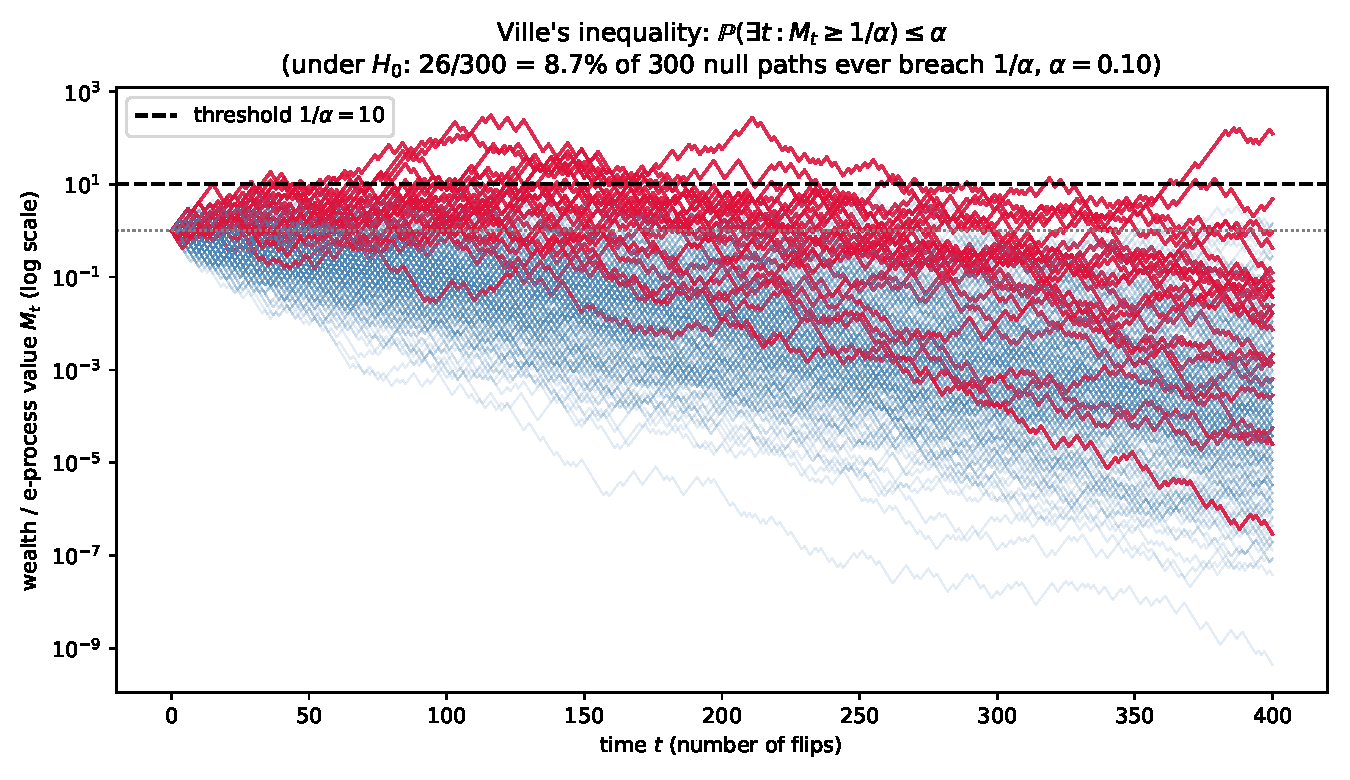
\includegraphics[width=0.62\textwidth]{ville_null.pdf}
\end{figure}

\framebreak

\begin{block}{Proposition 7.8: the converse}
Every level-$\alpha$ sequential test $\phi$ for $\mathcal P$ can be obtained by thresholding some e-process $M$ for
$\mathcal P$ at $1/\alpha$.
\end{block}

\textbf{Proof.} Define $M_t := \phi_t / \alpha$. Then $M_t$ only takes values $0$ or $1/\alpha$, so
$M_t \ge 1/\alpha \iff \phi_t = 1$. It remains to check $M$ is an e-process: for any stopping time $\tau$ and any
$\mathbb P \in \mathcal P$,
$$\mathbb{E}^{\mathbb P}[M_\tau] = \mathbb E^{\mathbb P}[\phi_\tau]/\alpha \le 1$$
by (7.2). $\blacksquare$

\textbf{Conclusion:} e-processes and level-$\alpha$ sequential tests are two sides of the same coin --- thresholding
one direction gives a test, and every test arises this way. But e-processes carry \emph{more} information (the
actual wealth/evidence value) than a binary reject/don't-reject decision, and remain interpretable without ever
thresholding.

\end{frame}

\begin{frame}{7.4 Optional continuation and p-processes}

\textbf{Intuition (optional continuation).} Suppose scientist A runs an experiment and produces e-process
$M^A$ up to some point (possibly a random, data-dependent point $\tau$). Scientist B can then take over,
starting a fresh e-process $M^B$ (with $M^B_t = 1$ while $t \le \tau$), and \emph{multiply} the two together. The
combined wealth is still a valid e-process --- evidence can be handed off between experimenters, or across looks,
without breaking validity.

\begin{block}{Proposition 7.9}
Let $M^A, M^B$ be e-processes for $\mathcal P$ and $\tau$ a stopping time with $M_t^B = 1$ on $\{t \le \tau\}$.
Define $M_t := M^A_{\tau\wedge t}\, M^B_t$. Then $M$ is an e-process for $\mathcal P$.
\end{block}

This means: switching betting strategies (even multiple times, even using human judgment about when to switch)
never invalidates the e-process, as long as each strategy is itself valid on its own turn.

\begin{block}{Definition 7.10: p-process}
A nonnegative process $P=(P_t)$ is a \emph{p-process} for $\mathcal P$ if $P_\tau$ is a p-variable for every
stopping time $\tau$ and every $\mathbb P \in \mathcal P$.
\end{block}

Ville's inequality (7.4a) immediately implies: if $M$ is an e-process, then $\big(\inf_{s\le t} 1/M_s\big)_{t}$ is a
p-process. Intuition: an e-process reports evidence \emph{now}; a p-process reports the \emph{best} evidence ever
seen so far --- which, like a company judged only by its best-ever quarter, tends to overstate performance.

\end{frame}

% ==========================================================================
\section{7.5 E-processes constructed from likelihood ratios}
% ==========================================================================

\begin{frame}{7.5.1 Log-optimality of the likelihood ratio process}

\textbf{Intuition.} If testing a simple $\mathbb P$ against a simple $\mathbb Q$, the natural e-process is just the
running likelihood ratio --- exactly the object from the SPRT. It turns out this is not just \emph{a} valid
e-process, it is the \emph{best possible} one, in a precise sense (log-optimality).

\begin{block}{Likelihood ratio process}
\begin{equation}
M_0 = 1, \qquad M_t = \prod_{i=1}^t \frac{\mathrm d\mathbb Q}{\mathrm d\mathbb P}(X_i) \quad \text{for } t\in\Nmb.
\tag{7.5}
\end{equation}
\end{block}
$M$ is not just an e-process, but a genuine \emph{test martingale} for $\mathbb P$ (even without the iid
assumption, using the running likelihood ratio of the first $n$ points).

\begin{block}{Theorem 7.11: log-optimality}
For any stopping time $\tau$ finite $\mathbb Q$-a.s., and any e-process $M'$ for $\mathbb P$,
\begin{equation}
\mathbb{E}^{\mathbb Q}[\log M_\tau] \ge \mathbb{E}^{\mathbb Q}[\log M'_\tau].
\tag{7.7}
\end{equation}
\end{block}
\emph{Proof idea:} $M'_\tau$ is measurable w.r.t.\ $\mathcal F_\tau$; for any $\mathbb P$-null event $A \in \mathcal
F_\tau$, one shows $\mathbb Q(A)=0$ too (using $\mathbb E^{\mathbb P}[\mathbb 1_A \mathbb 1_{\{\tau\le n\}} M_n]=0$
and taking $n\to\infty$), so $\mathbb Q \ll \mathbb P$ on $\mathcal F_\tau$; a general e-variable optimality result
(Proposition 3.22) then finishes the proof. No other e-process can beat the likelihood ratio's expected log-growth
at any stopping time.

\end{frame}

\begin{frame}[allowframebreaks]{7.5.2 Asymptotic log-optimality and the plug-in method}

\textbf{Intuition.} With iid data, the running likelihood ratio's growth rate settles down to a constant: the
Kullback--Leibler divergence $\mathrm{KL}(\mathbb Q,\mathbb P)$, by the law of large numbers. No e-process can grow
faster asymptotically.

\begin{block}{Proposition 7.12}
In the iid setting, the likelihood ratio process has asymptotic growth rate $\mathrm{KL}(\mathbb Q,\mathbb P) > 0$
(hence is consistent); no other e-process has a larger asymptotic growth rate.
\end{block}

\textbf{When $\mathbb Q$ is composite (unknown alternative):} plug in an estimate $\hat\theta_i$ of the alternative
parameter, updated online:
\begin{equation}
M_0=1, \qquad M_t = \prod_{i=1}^t \ell(X_i;\theta_i), \quad \theta_i \text{ measurable w.r.t.\ } \sigma(X_1,\dots,X_{i-1}).
\tag{7.8}
\end{equation}

\framebreak

\begin{block}{Definition 7.13: asymptotic log-optimality}
$M$ is asymptotically log-optimal for $\mathbb P$ against $\mathcal Q$ if for every $\mathbb Q \in \mathcal Q$,
$$\lim_{t\to\infty} \frac1t\big(\log M_t - \log M_t^{\mathbb Q}\big) \ge 0 \quad \text{in } L^1(\mathbb Q),$$
where $M^{\mathbb Q}$ is the (oracle) likelihood ratio process for $\mathbb Q$.
\end{block}

\begin{block}{Proposition 7.14 (sketch) and Corollary 7.15}
If $\log \ell(x;\theta)$ is concave in $\theta$ with gradient $\eta(x;\theta)$, and $\theta_i \to \theta$ in
$L^2(\mathbb Q_\theta)$ with $\sup_i \mathbb E^{\mathbb Q_\theta}[\|\eta(X_i;\theta_i)\|^2] < \infty$, then $M$ in
(7.8) is asymptotically log-optimal. \emph{Proof uses concavity to lower-bound the log-ratio gap by an inner
product, then Cauchy--Schwarz to show it vanishes.} E.g., for $\mathbb P = N(\theta_0,1)$ vs.\ $\mathbb Q_\theta =
N(\theta,1)$, using $\theta_i=$ running sample mean (the MLE) satisfies these conditions since
$\mathbb E^{\mathbb Q_\theta}[(\theta_i-\theta)^2] = 1/(i-1) \to 0$.
\end{block}

\end{frame}

% ==========================================================================
\section{7.6 Testing by betting}
% ==========================================================================

\begin{frame}{7.6 Testing by betting: the game}

\textbf{Intuition.} Recast the whole construction as a literal gambling game. The statistician (``Skeptic'') bets
on each new observation \emph{before} seeing it. Two requirements make this a valid test:
\begin{itemize}
\item[(a)] if the null is true, no strategy can make money \emph{systematically} (only by luck);
\item[(b)] if the null is false, some strategy \emph{can} guarantee long-run profit.
\end{itemize}
Final wealth (relative to the \$1 start) is then a direct, interpretable measure of evidence against the null.

\begin{block}{Algorithm 7.16: Testing by betting (simple null $\mathbb P$)}
\begin{enumerate}
\item[1.] Initial wealth $W_0 = 1$.
\item[2.] For $t=1,2,\dots$: choose bet $S_t : \mathcal X \to [0,\infty]$ with $\mathbb E^{\mathbb P}[S_t(X)\mid X_1,\dots,X_{t-1}] \le 1$.
\item[3.] Observe $X_t$; update $W_t = W_{t-1}\cdot S_t(X_t)$.
\end{enumerate}
\end{block}

The constraint on $S_t$ is exactly ``$S_t$ is a conditional e-variable for $\mathbb P$.'' This immediately makes
$W$ a test supermartingale for $\mathbb P$, for \emph{any} betting strategy satisfying the constraint.

\textbf{Optimal bet.} If the alternative $\mathbb Q$ is simple and $\mathbb P \ll \mathbb Q$, the exponent-optimal
bet (maximizing $\mathbb E^{\mathbb Q}[\log S_t]$ subject to the constraint) is exactly the conditional likelihood
ratio of $\mathbb Q$ to $\mathbb P$ --- recovering (7.5).

\end{frame}

\begin{frame}{7.6 Testing by betting: composite nulls}

\textbf{Intuition.} If the null is composite ($\mathcal P$ contains many candidate distributions), the statistician
must play a \emph{separate} game against every $\mathbb P \in \mathcal P$ simultaneously, and report the
\emph{worst-case} (most conservative) wealth across all these parallel games as the overall evidence.

\begin{block}{Algorithm 7.17: Testing by betting (composite null $\mathcal P$)}
\begin{enumerate}
\item[1.] For each $\mathbb P \in \mathcal P$: initial wealth $W_0^{\mathbb P}=1$.
\item[2.] For $t=1,2,\dots$: for each $\mathbb P$, choose $S_t^{\mathbb P}$ with
$\mathbb E^{\mathbb P}[S_t^{\mathbb P}(X)\mid X_1,\dots,X_{t-1}]\le1$.
\item[3.] Observe $X_t$; update $W_t^{\mathbb P} = W_{t-1}^{\mathbb P}\cdot S_t^{\mathbb P}(X_t)$ for each $\mathbb P$.
\item[4.] Overall wealth: $W_t = \inf_{\mathbb P\in\mathcal P} W_t^{\mathbb P}$.
\end{enumerate}
\end{block}

This is only an \emph{interpretation} --- we never literally instantiate uncountably many parallel games in
practice; sensible e-processes for composite nulls are usually built more directly (Sections 7.7--7.9). But the
betting picture is what makes e-processes intuitive as ``evidence,'' and clarifies why e-processes generalize test
supermartingales.

\end{frame}

\begin{frame}[allowframebreaks]{Running example: sequentially testing a coin's fairness}

\textbf{Setup.} $H_0: \theta = 0.5$ (fair coin). We bet using the fixed likelihood-ratio strategy towards
$q = 0.6$: multiply current wealth by $1.2$ on heads, by $0.8$ on tails. We generate an actual sequence of 30 coin
flips (seeded pseudo-randomly, true bias $p=0.6$) and track wealth $W_t$ after each flip.

\textbf{The 30 simulated flips} (1 = heads, 0 = tails; 19 heads observed):
$$0,1,1,1,0,0,0,1,1,1,1,1,1,1,0,1,1,1,0,1,0,0,1,1,0,1,1,1,0,0$$

\framebreak

\begin{table}
\centering
\scriptsize
\begin{tabular}{crc @{\hspace{1.2cm}} crc @{\hspace{1.2cm}} crc}
\toprule
$t$ & flip & $W_t$ & $t$ & flip & $W_t$ & $t$ & flip & $W_t$ \\
\midrule
1  & T & 0.800 & 11 & H & 1.468 & 21 & T & 2.693 \\
2  & H & 0.960 & 12 & H & 1.761 & 22 & T & 2.154 \\
3  & H & 1.152 & 13 & H & 2.113 & 23 & H & 2.585 \\
4  & H & 1.382 & 14 & H & 2.536 & 24 & H & 3.102 \\
5  & T & 1.106 & 15 & T & 2.029 & 25 & T & 2.481 \\
6  & T & 0.885 & 16 & H & 2.435 & 26 & H & 2.978 \\
7  & T & 0.708 & 17 & H & 2.922 & 27 & H & 3.573 \\
8  & H & 0.849 & 18 & H & 3.506 & 28 & H & 4.288 \\
9  & H & 1.019 & 19 & T & 2.805 & 29 & T & 3.430 \\
10 & H & 1.223 & 20 & H & 3.366 & 30 & T & 2.744 \\
\bottomrule
\end{tabular}
\caption{\scriptsize Wealth $W_t$ after each of 30 simulated flips ($1.2\times$ on heads, $0.8\times$ on tails).}
\end{table}

\framebreak

\textbf{What if we stop early at flip 12 vs.\ continue to flip 30?}
\begin{itemize}
\item At $t=12$: wealth $W_{12} = 1.761$. If we report evidence here and stop, this is a perfectly valid e-value:
$\mathbb E^{\mathbb P}[W_{12}] \le 1$ under $H_0$, by construction.
\item If instead we continue to $t=30$: wealth $W_{30} = 2.744$. This is \emph{also} a perfectly valid e-value at
its own stopping time.
\item \textbf{Key point:} both are valid \emph{simultaneously}, for \emph{any} stopping rule we might have used to
decide between them (even a rule based on how the wealth looked at $t=12$!). This is exactly Ville's inequality /
optional stopping at work: $\mathbb P(\exists t \le 30 : W_t \ge 1/\alpha) \le \alpha$ regardless of which $t$ we
end up choosing.
\item Notice wealth is \emph{not} monotonic --- it dips (e.g., $t=5$--$7$, down to $0.708$) before recovering. A
classical $p$-value process peeked at those dips would look ``worse than random,'' but the e-process framework
does not care: only the value at the (possibly random) time you actually stop matters, and the guarantee holds
regardless.
\item At $\alpha = 0.05$ (threshold $1/\alpha = 20$), we never come close to rejecting with this particular random
sequence --- consistent with $H_0$ being em true and $q=0.6\ne \theta_1=0.5$ giving only modest average growth
per step under $H_0$ in expectation (growth here is due to the true bias being $p=0.6$, matching our bet).
\end{itemize}

\end{frame}

\begin{frame}[fragile]{Python: testing-by-betting simulation (the coin example)}

\begin{lstlisting}
import numpy as np

def betting_wealth(flips, q=0.6):
    """flips: list of 0/1 (tails/heads). Bet towards alternative q."""
    wealth = [1.0]
    for x in flips:
        factor = 2*q if x == 1 else 2*(1-q)
        wealth.append(wealth[-1] * factor)
    return wealth

rng = np.random.default_rng(42)
flips = [1 if rng.random() < 0.6 else 0 for _ in range(30)]
wealth = betting_wealth(flips, q=0.6)

for t, (x, w) in enumerate(zip(flips, wealth[1:]), start=1):
    print(f"t={t:2d}  flip={'H' if x else 'T'}  W_t={w:.3f}")

alpha = 0.05
threshold = 1/alpha
print("Stop at t=12, wealth =", round(wealth[12], 3))
print("Continue to t=30, wealth =", round(wealth[30], 3))
print("Reject H0 at level", alpha, "?", any(w >= threshold for w in wealth))
\end{lstlisting}

\end{frame}

% ==========================================================================
\section{7.7 The universal inference e-process}
% ==========================================================================

\begin{frame}[allowframebreaks]{7.7 The universal inference e-process}

\textbf{Intuition.} We want an e-process even when $\mathcal P$ is composite and no nontrivial test martingale
family may exist. Idea: compare an \emph{out-of-sample} alternative likelihood to an \emph{in-sample} (i.e.,
overfit) null likelihood. Overfitting under the null only \emph{helps} validity (it can only shrink the ratio), so
this is safe.

\begin{block}{Universal inference e-process (7.9)}
$$E_0=1,\qquad E_t = \prod_{i=1}^t \frac{\hat q_{i-1}(X_i)}{\hat p_t(X_i)},$$
where $\hat q_{i-1}\in\mathcal Q$ may depend on $X_1,\dots,X_{i-1}$ (updated online), and $\hat p_t \in \mathcal P$
is the MLE in $\mathcal P$ based on \emph{all} of $X_1,\dots,X_t$ (recomputed every step).
\end{block}

\begin{block}{Proposition 7.18}
$E$ in (7.9) is an e-process for $\mathcal P$.
\end{block}
\emph{Proof idea:} by definition of the MLE $\hat p_t$, for every fixed $\mathbb P \in \mathcal P$ with density $p$,
$$E_t \le \prod_{i=1}^t \frac{\hat q_{i-1}(X_i)}{p(X_i)} =: (\text{test martingale for } \mathbb P),$$
since $\hat p_t$ maximizes the denominator (over $\mathcal P$) using the very same data, so replacing it with the
true $p$ can only make the ratio $\ge E_t$. The right side is a genuine test martingale for $\mathbb P$ (product
of conditional likelihood ratios), which certifies $E$ as an e-process.

\framebreak

\textbf{Ratio interpretation:} $\dfrac{\text{out-of-sample alternative likelihood}}{\text{in-sample null likelihood}}$.
Each $\hat q_{i-1}$ is evaluated on a fresh point $X_i$ outside the sample used to fit it; $\hat p_t$ is evaluated
on all the data used to fit it. We ``overfit'' the null (safe) but not the alternative (would be unsafe). This
avoids the complexity-adjustment headaches of generalized likelihood ratio tests, where thresholds must be enlarged
to account for $\mathcal P,\mathcal Q$ complexity --- here the threshold $1/\alpha$ never needs adjusting. A
mixture variant, $E_t = \int_{\mathcal Q} \prod_i \frac{q(X_i)}{\hat p_t(X_i)}\,\mathrm d\nu(q)$, is also an
e-process.

\end{frame}

% ==========================================================================
\section{7.8 Sequential e-values and empirically adaptive e-processes}
% ==========================================================================

\begin{frame}[allowframebreaks]{7.8 Sequential e-values}

\textbf{Intuition.} Imagine a chain of independent laboratories, lab $1, 2, 3, \dots$, each producing one e-value
$E_t$ using only the results $E_1,\dots,E_{t-1}$ reported by earlier labs (plus its own new data). Each lab's e-value
is valid \emph{conditionally} on everything reported before it. Multiplying all these e-values together builds
a full e-process --- evidence accumulates multiplicatively and validly across the whole chain.

\begin{block}{Definition 7.19: sequential e-values}
E-variables $E_t$, $t \in \mathbb T_+$, adapted to $\mathcal F$, are \emph{sequential} if
$$\mathbb E^{\mathbb P}[E_t \mid \mathcal F_{t-1}] \le 1 \quad \text{for all } t\in\mathbb T_+,\ \mathbb P\in\mathcal P.$$
(Default filtration: natural filtration of the $E_t$'s themselves.)
\end{block}

\begin{block}{Proposition 7.20}
If $(E_t)_{t\in\mathbb T_+}$ are sequential e-variables for $\mathcal P$, then $M_t := \prod_{s=1}^t E_s$
(with $M_0=1$) is an e-process for $\mathcal P$.
\end{block}
\emph{Proof:} $\mathbb E^{\mathbb P}[M_t\mid\mathcal F_{t-1}] = M_{t-1}\,\mathbb E^{\mathbb P}[E_t\mid\mathcal
F_{t-1}] \le M_{t-1}$, so $M$ is a test supermartingale, hence an e-process.

\framebreak

\textbf{Betting on sequential e-values.} Rather than betting \emph{everything} on each $E_t$ (fully multiplying),
we can bet only a \emph{fraction} $\lambda_t \in [0,1]$ of wealth --- convex-combining ``do nothing'' (factor 1)
and ``bet fully'' (factor $E_t$).

\begin{block}{Definition 7.21: e-process built on sequential e-values}
\textbf{(i)} \begin{equation}
M_t = \prod_{s=1}^t \big((1-\lambda_s) + \lambda_s E_s\big), \quad M_0=1,
\tag{7.10}
\end{equation}
where $\lambda_t\in[0,1]$ is predictable (a measurable function of $E_1,\dots,E_{t-1}$).

\textbf{(ii)} The $\mathbb Q$-\emph{log-optimal} choice solves
$\lambda_t \in \arg\max_{\lambda\in[0,1]} \mathbb E^{\mathbb Q}[\log((1-\lambda)+\lambda E_t)\mid \mathcal F_{t-1}]$.

\textbf{(iii)} The \emph{empirically adaptive} e-process (parameter $\gamma\in(0,1]$) instead solves, for $t\ge2$,
$$\lambda_t \in \arg\max_{\lambda\in[0,\gamma]} \frac{1}{t-1}\sum_{s=1}^{t-1}\log\big((1-\lambda)+\lambda E_s\big), \qquad \lambda_1=0,$$
i.e., $\lambda_t$ is chosen using only the \emph{empirical} track record of past e-values, with no need to know a
specific alternative $\mathbb Q$.
\end{block}

\framebreak

\textbf{Interpretation.} The $\mathbb Q$-log-optimal choice maximizes ``e-power'' at each step assuming you know
$\mathbb Q$; the empirically adaptive choice mimics this using only the empirical distribution of past e-values ---
a purely data-driven analogue with a default choice $\gamma = 1/2$. This construction is always a supermartingale
(and a martingale if the $E_t$ are exact), and $M_\tau$ is a valid e-variable at any stopping time $\tau$.

\begin{block}{Theorem 7.22}
Suppose $(E_t)_{t\in\Nmb}$ are iid under $\mathbb Q$ with $\mathbb E^{\mathbb Q}[\log E_1]$ finite. The empirically
adaptive e-process $M$ (with $\gamma=1$) satisfies:
\begin{enumerate}
\item[(i)] \emph{Asymptotic log-optimality:} $\lim_{t\to\infty}\frac1t(\log M_t - \log M'_t) \ge 0$ in
$L^1(\mathbb Q)$, where $M'$ is the $\mathbb Q$-log-optimal e-process built on the same $(E_t)$.
\item[(ii)] \emph{Consistency:} if $\mathbb E^{\mathbb Q}[E_1] > 1$, then $M_t \to \infty$, $\mathbb Q$-almost surely.
\end{enumerate}
\end{block}
\emph{Proof intuition:} under the iid assumption, $\lambda_t$ converges in probability to the fixed optimal
$\lambda^*$ that would be chosen with full knowledge of $\mathbb Q$; the two e-processes then share the same
asymptotic growth rate by the law of large numbers.

\end{frame}

\begin{frame}[fragile]{Python: testing-by-betting with sequential e-values (empirically adaptive)}

\begin{lstlisting}
import numpy as np

def empirically_adaptive(E, gamma=0.5):
    """E: array of sequential e-values E_1,...,E_T. Returns wealth M_0,...,M_T."""
    T = len(E)
    M = [1.0]
    lam = 0.0  # lambda_1 = 0
    log_growth_hist = []  # to average over E_1,...,E_{t-1}
    for t in range(T):
        M.append(M[-1] * ((1 - lam) + lam * E[t]))
        log_growth_hist.append(E[t])
        # choose lambda_{t+2} by grid search maximizing empirical mean growth
        grid = np.linspace(0, gamma, 200)
        avg_log = [np.mean(np.log((1 - l) + l * np.array(log_growth_hist))) for l in grid]
        lam = grid[int(np.argmax(avg_log))]
    return np.array(M)

rng = np.random.default_rng(0)
# Sequential e-values under an alternative where E[E_t] = 1.5 (favorable game)
E_vals = rng.exponential(scale=1.5, size=200)
M = empirically_adaptive(E_vals, gamma=0.5)
print("Final wealth after 200 rounds:", round(M[-1], 3))
print("Wealth path (every 20 steps):", np.round(M[::20], 3))
\end{lstlisting}

\end{frame}

% ==========================================================================
\section{7.9 Obtaining an e-process from e-values using time-mixture}
% ==========================================================================

\begin{frame}[allowframebreaks]{7.9 Time-mixture construction}

\textbf{Intuition.} Suppose at every sample size $n$ you have a good e-variable $E^{(n)}$ (a ``numeraire''), each
individually valid, but the \emph{sequence} $E^{(1)}, E^{(2)}, \dots$ is not necessarily an e-\emph{process} (e.g.,
these could be entirely different statistics recomputed from scratch at each $n$, with no consistency across $n$).
We can still combine them into a bona fide e-process by taking a weighted average across time --- putting a
probability distribution over ``which $n$ do I trust most,'' and never re-normalizing.

\begin{block}{Time-mixture e-process (7.12)}
Let $w$ be any probability mass function on $\Nmb=\{1,2,\dots\}$. Define $M_0=1$ and
$$M_n = \sum_{j\le n} w(j)\, E^{(j)}.$$
\end{block}

\begin{block}{Proposition 7.23}
$M$ defined above is an e-process for $\mathcal P$.
\end{block}

\framebreak

\emph{Proof:} for any random time $\tau$ (not even required to be a stopping time!) and any $\mathbb P \in \mathcal
P$,
$$\mathbb E^{\mathbb P}[M_\tau] = \mathbb E^{\mathbb P}\Big[\sum_{j\ge1} w(j) E^{(j)} \sum_{n\ge j} \mathbb 1_{\{\tau=n\}}\Big]
\le \sum_{j\ge1} w(j)\,\mathbb E^{\mathbb P}[E^{(j)}] \le 1,$$
using $\sum_{n\ge j}\mathbb 1_{\{\tau=n\}} \le 1$ and each $E^{(j)}$ being an e-variable.

\textbf{Practical weight choice.} $w(n) = c/(n(\log n)^2)$ (normalized so weights sum to 1) gives
$\log M_n \ge \log E^{(n)} - \log n - 2\log\log n - O(1)$, so
$$\lim_{n\to\infty}\Big(\tfrac1n\log M_n - \tfrac1n\log E^{(n)}\Big) = 0:$$
the time-mixed e-process matches the asymptotic growth rate of the underlying numeraire sequence, at essentially no
cost.

\end{frame}

\begin{frame}[fragile]{Python: time-mixture construction}

\begin{lstlisting}
import numpy as np

def time_mixture_weights(n_max):
    # w(n) = c / (n (log n)^2) for n>=2, normalized; w(1) fills remaining mass
    n = np.arange(2, n_max + 1)
    raw = 1.0 / (n * (np.log(n)) ** 2)
    w = np.zeros(n_max + 1)
    w[2:] = raw / raw.sum() * 0.99
    w[1] = 1 - w.sum()
    return w

def time_mixture_eprocess(E, w):
    # M_n = sum_{j<=n} w(j) E^(j); E[j-1] holds numeraire E^(j)
    return np.cumsum(w[1:len(E)+1] * E)

n_max = 500
w = time_mixture_weights(n_max)

# E^(n): fixed-n numeraire growing like exp(0.05 n) under the alternative
rng = np.random.default_rng(3)
logE = 0.05 * np.arange(1, n_max + 1) + rng.normal(0, 0.3, size=n_max)
E = np.exp(logE)

M = time_mixture_eprocess(E, w)
print("Growth rate of E^(n):", round(logE[-1] / n_max, 4))
print("Growth rate of M_n:  ", round(np.log(M[-1]) / n_max, 4))
\end{lstlisting}

\end{frame}

% ==========================================================================
\section{7.10 E-processes avoid reasoning about hypothetical worlds}
% ==========================================================================

\begin{frame}[allowframebreaks]{7.10 A quantum-like puzzle for p-values}

\textbf{The conceptual point.} Whether a $p$-value is ``valid'' can depend not just on what actually happened, but
on what \emph{would have happened} in hypothetical alternate runs of the experiment that never occurred. E-processes
never have this problem: validity only depends on the actual stopping time you actually used, because \emph{every}
stopping time is simultaneously valid.

\begin{block}{Example 7.24 (paraphrased): Bob and Alice}
Bob runs an A/B test intending to collect 10{,}000 observations. He looks once at 5000 points (but does not stop),
then continues to 10{,}000 and reports $p=0.04$. His boss Alice asks: ``If you had seen $>4800$ tails in the first
5000 tosses, what would you have done?'' Bob admits he would have stopped early. Alice says this makes his reported
$p=0.04$ \emph{invalid}: because Bob's actual stopping rule was implicitly data-dependent (sometimes 5000, sometimes
10{,}000, depending on a hypothetical world that never happened), the fixed-$n=10{,}000$ $p$-value calculation no
longer applies.
\end{block}

\framebreak

\textbf{Why this is unsettling.} The validity of Bob's $p$-value in the \emph{actual, realized} world depends on
his hypothetical answer about a world that did \emph{not} occur. Merely being asked ``what if'' --- and answering
honestly --- retroactively changes whether his real result is valid. This is impractical (nobody can enumerate
all such counterfactuals) and conceptually troubling.

\begin{block}{The e-process resolution}
If Bob instead reports $E_{10{,}000}$ from a genuine e-\emph{process} $(E_n)_{n\in\Nmb}$ (not just a sequence of
e-values), then \textbf{both} $5000$ and $10{,}000$ are valid stopping times \emph{simultaneously}, by construction
of e-processes (Ville's inequality holds uniformly over all stopping times). It does not matter what Bob
\emph{would} have done in a hypothetical world at $n=5000$ --- whatever he would have reported there would also
have been valid. There is no interference between hypothetical and actual worlds.
\end{block}

\textbf{Takeaway.} E-processes let you reason \emph{forward only}, using just the data you actually observed and
the stopping time you actually used --- with no need to imagine what you would have done under alternate
hypothetical stopping rules. This is a conceptual, not just technical, advantage of e-processes over $p$-values
under optional stopping.

\framebreak

\begin{figure}
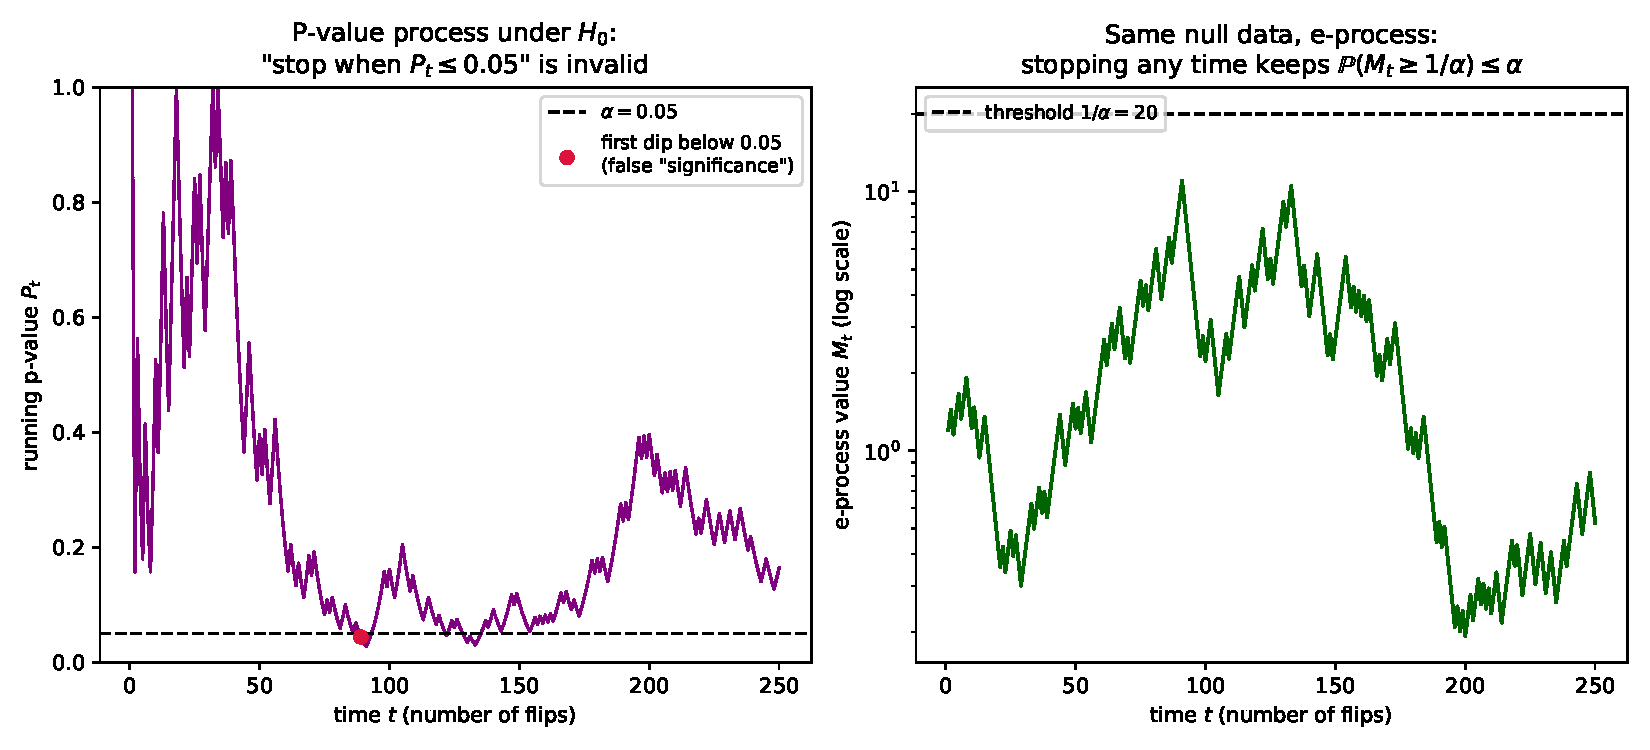
\includegraphics[width=0.92\textwidth]{optional_stopping.pdf}
\end{figure}
\textbf{Left:} under a true null, the running $p$-value process can dip below $0.05$ purely by chance at some
intermediate time --- ``stop whenever $P_t \le 0.05$'' is an invalid procedure. \textbf{Right:} the corresponding
e-process, built from the same data, stays comfortably under the threshold $1/\alpha$; stopping at \emph{any} time
(this one or any other) keeps $\mathbb P(M_t \ge 1/\alpha) \le \alpha$ exactly as Ville's inequality guarantees.

\end{frame}

% ==========================================================================
\section{7.11 A pathological example for the e-power of e-processes}
% ==========================================================================

\begin{frame}[allowframebreaks]{7.11 When e-power misleads}

\textbf{Intuition.} ``E-power'' (expected log-growth, $\mathbb E^{\mathbb Q}[\log M_t]$) has been our main
optimality criterion. This section shows two cautionary, somewhat pathological examples where e-power gives a
\emph{wrong impression} of an e-process's actual performance, because of subtleties with infinite expectations.

\textbf{Two possible failure modes:}
\begin{itemize}
\item[(a)] an e-process can have \emph{positive infinite} e-power at each fixed time, yet decline to $0$ with
probability 1 under $\mathbb Q$;
\item[(b)] an e-process can have \emph{negative infinite} e-power at each fixed time, yet increase to $\infty$ with
probability 1 under $\mathbb Q$.
\end{itemize}
Moral: extra caution is needed whenever infinities appear in e-power calculations.

\framebreak

\begin{block}{Example 7.25}
Let $E_t = \exp(t^2 - Y_t)$, $t\in\Nmb$, be e-variables for $\mathbb P$ ($\mathbb E^{\mathbb P}[E_t]\le1$), where
$Y_1,Y_2,\dots$ are iid $\mathrm{Pareto}(1)$ under $\mathbb Q$ (i.e., $\mathbb Q(Y_1 > x) = 1/x$ for $x \ge 1$),
independent under $\mathbb P$. Let $M_t = \prod_{s=1}^t E_s$ (an e-process by Proposition 7.20).

One shows, for any $x > 0$,
$$\mathbb Q(M_t \le x) = \mathbb Q\Big(\sum_{s=1}^t Y_s \ge \tfrac{t(t+1)(2t+1)}{6} - \log x\Big) \le t\,\mathbb Q\Big(Y_1 \ge \tfrac{(t+1)(2t+1)}{6} - \tfrac{\log x}{t}\Big) \to 0$$
as $t \to \infty$ (using a union bound and $\mathbb Q(Y_1 > x) = 1/x \to 0$). So $M_t \to \infty$ in
$\mathbb Q$-probability --- thresholding $M_t$ rejects the null with probability approaching 1!

\textbf{But:} because $\mathrm{Pareto}(1)$ has infinite mean ($\mathbb E^{\mathbb Q}[Y_1] = \infty$),
$$\mathbb E^{\mathbb Q}[\log E_t] = t^2 - \mathbb E^{\mathbb Q}[Y_t] = t^2 - \infty = -\infty \quad \text{for every } t,$$
so $\mathbb E^{\mathbb Q}[\log M_t] = -\infty$ for every $t$ --- the exact same (uninformative) e-power as the
useless \emph{zero} process, despite $M$ being a highly effective test in practice!
\end{block}

\framebreak

\begin{block}{Example 7.26 (general phenomenon)}
If $E_1,E_2,\dots$ are independent e-variables for $\mathbb P$, and $E_1$ satisfies
$\mathbb E^{\mathbb Q}[\log E_1] = -\infty$ (as in Example 7.25) while every $E_t$, $t\ge2$, has finite e-power,
then $M_t = \prod_{s=1}^t E_s$ satisfies $\mathbb E^{\mathbb Q}[\log M_t] = -\infty$ for \emph{every} $t$ --- no
matter how favorably $M$ grows after time 1. One can easily arrange $M_t \to \infty$ in $\mathbb Q$-probability
regardless.
\end{block}

\framebreak

\textbf{The mirror image.} Taking reciprocals in Examples 7.25--7.26 produces e-processes with \emph{positive
infinite} e-power at every fixed time, that nonetheless \emph{decline to 0} with probability 1 under $\mathbb Q$
--- the opposite pathology. Both directions show that e-power, while a useful guiding criterion throughout this
book, must be interpreted carefully whenever infinite expectations are in play; finite-sample or probabilistic
(not just expectation-based) criteria remain essential complements.

\end{frame}

% ==========================================================================
\section{Summary}
% ==========================================================================

\begin{frame}[allowframebreaks]{Chapter 7 summary}

\begin{itemize}
\item \textbf{Peeking at $p$-values} (7.1) is dangerous: stopping when $P_n\le\alpha$ can force
$\mathbb P(P_\tau\le\alpha)=1$ under the null (``sampling to a foregone conclusion'').
\item \textbf{Wald's SPRT} (7.2) shows sequential testing can be far more efficient than fixed-$n$ testing, while
foreshadowing the e-process machinery (the likelihood ratio process).
\item \textbf{Test supermartingales and e-processes} (7.3) formalize ``wealth that cannot systematically grow under
the null'': e-processes are the more general, more flexible notion, equivalent to being dominated by a test
martingale family.
\item \textbf{Ville's inequality} (7.4) is the time-uniform generalization of Markov's inequality: $\mathbb
P(\exists t: M_t\ge1/\alpha)\le\alpha$. It converts e-processes into level-$\alpha$ sequential tests, and every
such test arises this way (Proposition 7.8).
\item \textbf{Likelihood ratio processes} (7.5) are exactly log-optimal e-processes for simple nulls/alternatives,
and asymptotically log-optimal (via plug-in estimation) for composite alternatives.
\item \textbf{Testing by betting} (7.6) reframes all of this as a literal gambling game --- wealth is evidence.
\item \textbf{Universal inference} (7.7) builds e-processes for composite nulls via out-of-sample
alternative-likelihood over in-sample null-likelihood (MLE) ratios.
\item \textbf{Sequential e-values} (7.8) can be multiplied, or fractionally bet on via $(1-\lambda)+\lambda E_t$,
to build e-processes; the empirically adaptive choice of $\lambda_t$ needs no knowledge of the alternative.
\item \textbf{Time-mixture} (7.9) converts any sequence of per-$n$ e-variables (numeraires) into a genuine
e-process via a simple weighted sum, at negligible cost to asymptotic growth rate.
\item \textbf{E-processes avoid hypothetical-world reasoning} (7.10): unlike $p$-values under optional stopping,
their validity never depends on what you \emph{would have} done in an alternate, unrealized run.
\item \textbf{E-power has pathologies} (7.11): infinite expectations can make e-power wildly misleading; probabilistic
convergence statements are an essential complement.
\end{itemize}

\end{frame}

\end{document}
